% Michal Kovac's master thesis
%
\documentclass{article}
\usepackage{pgf}

\pgfdeclareimage[interpolate=true,height=7cm]{faktorial}{faktorial}
\pgfdeclareimage[interpolate=true,height=7cm]{designimage}{designB}
\pgfdeclareimage[interpolate=true,height=3cm]{designimageSmall}{designB}
\pgfdeclareimage[interpolate=true,height=3.5cm]{creatorFactoryimage}{creatorFactory}

\author{Michal Kov\'{a}\v{c}}
\title{User oriented language for powerful data mining with Ferda}
\date{\today}

\begin{document}
\section{Introduction}
\subsection{History}
GUHA method

LISp-Miner

Michal Kov\'{a}\v{c}, Tom\'{a}\v{s} Kucha\v{r}, Alexander Kuzmin and Martin Ralbovsk\'{y} have started to work on the Ferda Data Miner in the year 2003. The project lead was Jan Rauch. The basic aim of this project had to be creating of a user friendly user interface for the LISp-Miner project. It was achieved, but the Ferda was created in mind of future extensions and main parts of the application are independend on data mining at all.

Ferda is user orieted application for working with special objects called boxes. Boxes have sockets and a user can connect to these sockets another boxes. Boxes have functions, sockets are places for parameters for these functions. The Ferda Data Miner is Ferda with boxes for data mining.

First boxes for data mining were written for LISp-Miner generators. It was hardly extensible. Later Tom\'{a}\v{s} Kucha\v{r} as part of his diploma thesis written own implementation of basic GUHA procedures for the Ferda Data Miner.

There are many new boxes created for special applications like decission trees, ontology mapping or relational data mining.

\section{Ferda Data Miner}
\subsection{Implementation}

Base parts of Ferda has been written in C\# 2.0. Ferda runs on both .NET Framework and Mono. Some parts of new boxes use also Java platform. Ferda uses middleware Internet Communications Engine for communication between its parts. Every part can be written in another language and run on another computer. For easier developement many third party libraries and application have been used -- mainly NAnt, NUnit, NDoc, Netron Graphic Library and DockDotNet. 

Ferda is under second version of General Public License. It allows everybody to use it for free, redistibute it, change the code if a result will be still under the General Public License.

Aim was to create application which is internationalized, well documented, modular, user friendly and conforms microsoft standards in user experience.

Ferda is client-server application. Client executable is FerdaFrontEnd.exe and we call that part FrontEnd. There isn't one server executable instead there are more separate modules which all can act as separate applications. FrontEnd comunicates with all of them. Some of these modules implements boxes so we call them box modules, other are helper modules like GUHA mining engine.

\noindent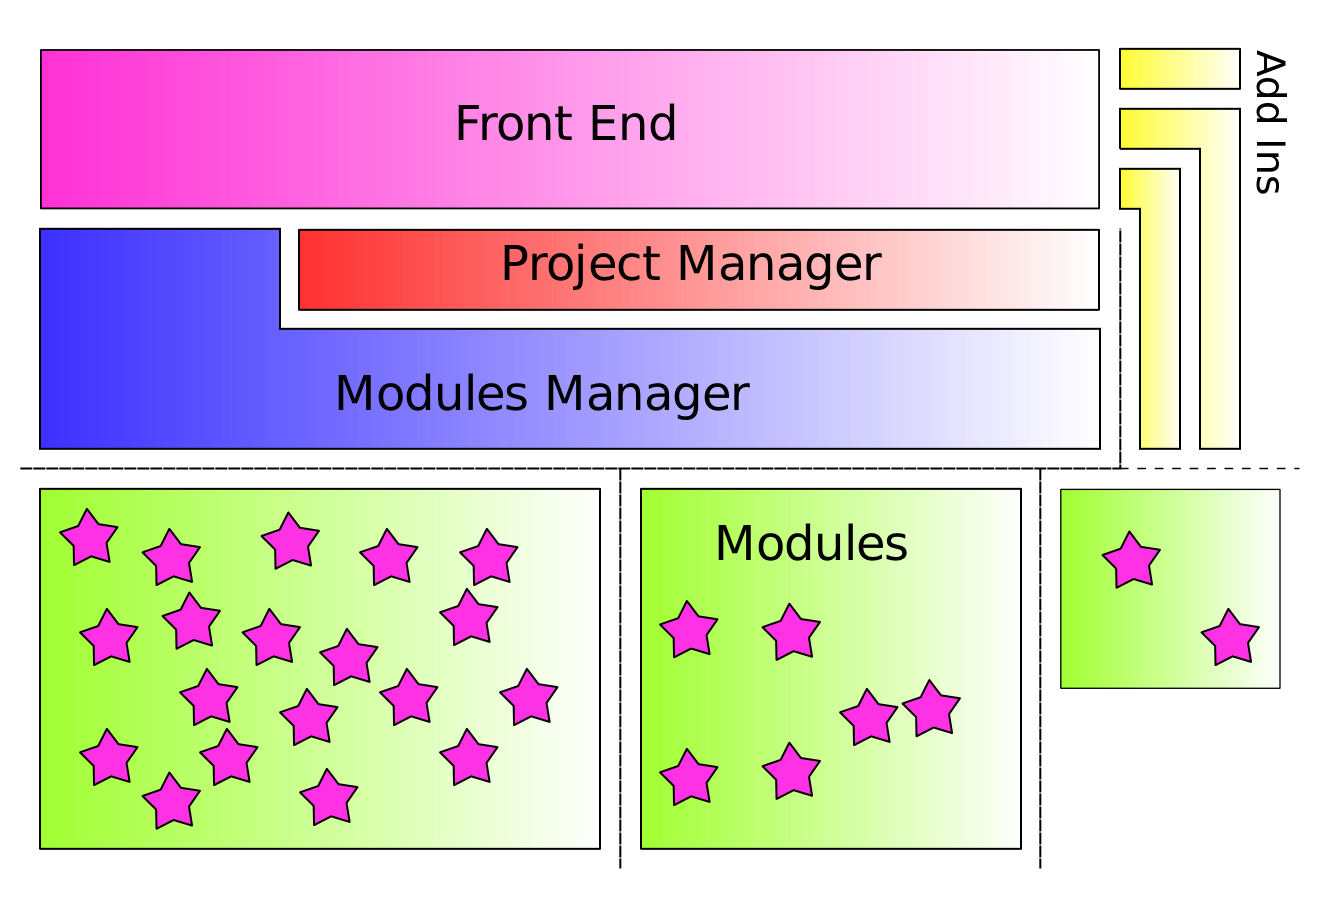
\includegraphics[width=12cm]{designB}

FrontEnd uses assembly FerdaModulesManager.dll for communicating with modules. This assembly is layer of abstraction so that FrontEnd does not know that modules are not implemented localy.

Another assembly that is used by FrontEnd is FerdaProjectManager.dll. It obhospodaruje projects. Project consists of box instances which are placed in an archive and views. Views adds to boxes its placement on a desktop. This manaher is able to load project from xml file and save it to xml file.

FrontEnd also loads add ins. Add ins can extend functionality of FrontEnd in many ways. Mainly it is used for modules for interaction and setting modules. Modules for interaction work on top of some box module. It for example show results of functions returned by the box module. Setting modules are used for helping with setting nonstandard properties.

Comunucation between FrontEnd and modules and between modules itself are done be Internet Communication Engine (ICE). ICE is strong modern middleware. Thanks to usage of ICE Ferda is language and framework independend and it allow as to run different modules on different computers, but it doesn't add big complexity to the application. It can be also used for distributed computing.

IceGrid applications, which manages available modules and loads them on demand, runs on a network. Modules manager uses these application for getting modules.

Every box module implementation has it's factory class. This factory class creates box module instances. There is one more layer -- every box module factory has it's factory class, we call it box module factory creator. It is used as singleton.

\noindent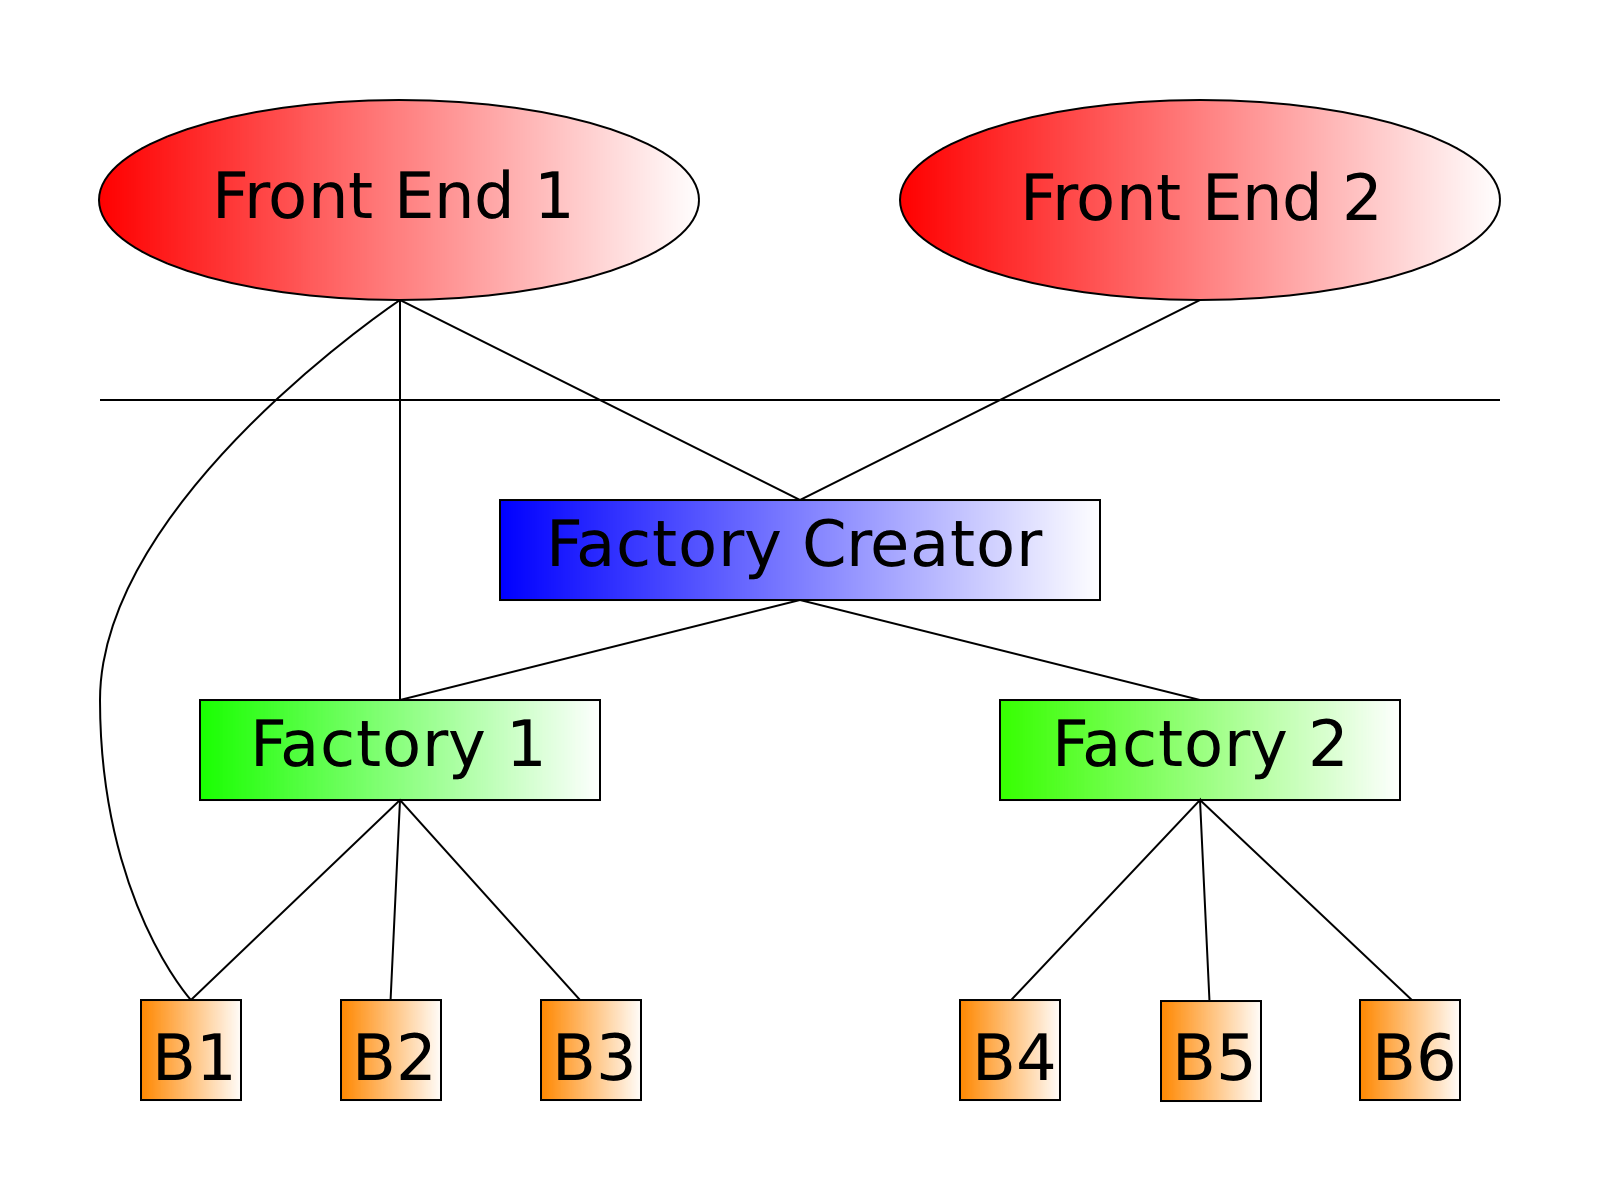
\includegraphics[width=12cm]{creatorFactory}

FrontEnd asks box module factory creator for creation of only one box module factory for one box class. Creator has methods independend on both instance of box module and FrontEnd connected and factory has methods independend on box modules, but dependend on FrontEnd (for example localized names of properties). When FrontEnd is not connected for longer time all factory instances and box module instances are destroyed.

Box modules mainly consists of sockets, properties and functions. Sockets are places where you can connect another box module. They are parameters for functionality of the box module. Properties are also parameters and can be viewed as socket, but can be configured both by connecting a box to the socket and by setting the property in the property grid.

Functions is some class which box returns. This class represents the functionality of a box.

Box module has also identifier, icon, svg design, names of categories, box modules asking for creation, actions, name of property driving label and dynamic help.

\subsection{Ferda as programming language}
The main concept of Ferda is to be user oriented functional language. Basic view is that a box is a function and sockets are properties of that function. There is no need to talk about properties, because properties are also usable by sockets. To be more precise, box can be not only viewed as one function, but as set of functions. As was writen box returns class as functions. So every method of such class can be viewed as separate function. Box can also return diferrent functions class depending on its parameters. 

Box is $\left<S,F\right>$ where
\begin{itemize}
	\item $S$ is a set of sockets
	\item $F$ is a set of functions
\end{itemize}
	
Socket is $\left<n,T\right>$ where
\begin{itemize}
	\item $n$ is socket name
	\item $T$ is a set of box types
\end{itemize}

We have prediate $has(f,i)$ where $f$ is function and $i$ is ``Ice identifier''

Type is $\left<i,S\right>$ where
\begin{itemize}
	\item $i$ is ``Ice identifier''
	\item $S$ is a set of $\left<n,i\right>$
	\begin{itemize}
		\item $n$ is socket name
		\item $i$ is ``Ice identifier''
	\end{itemize}
\end{itemize}

Box $B=\left<S,F\right>$ is of type $A=\left<i,Z\right>$ iff 
\begin{enumerate}
	\item $(\forall \left<n,j\right>\in Z)(\exists \left<m,T\right>\in S)(\exists \left<y,W\right>\in T)(m=n \wedge j=y)$
	\item $(\exists f\in F)(has(f,i))$
\end{enumerate}
	
\begin{itemize}
	\item Box consists of functions
	\item Sockets are parameters of these functions
	\item Property is also socket
		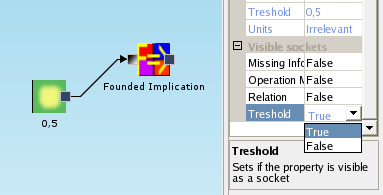
\includegraphics[width=7cm]{property_as_socket}
\end{itemize}

What is missing?
\begin{itemize}
	\item Moving work from one project to another
	\item Basic math boxes
	\item Recursion
	\item Other language boxes
	\item Ferda specific language boxes
	\item Data mining specific boxes for user programming
\end{itemize}

\section{Lambda calculus}
Base of functional languages is in lambda calculus. 

%rekurzivne spocetny
%vsecno je funkce
%typovany/netypovany
\section{Functional languages}
%prvky - vzhledem k Ferdovi
%jak delaji rekurzi / lambdu - rozsil mezi structuralnim a funkcionalnim jazykem

\section{Making things better in actual implementation}
\section{Reusability}
Ever programming languages have ways how to reuse a code. 

\subsection{Project import}
The simliest way is to copy the source code to different place and use it for different project. The same is possible in Ferda, you can copy a project file and reuse it.

With standard textual source code it is easy to merge the code from more sources. You can do it with Ferda project, but you must merge a code in a project files manualy in a text editor. The merging is not an easy process so it is not so much user friendly way.

It would be nice have a functionality in Ferda that will allow us to import some or all boxes from one project into another one. One way how to achieve that is adding a new item "import project\dots" to the ferda menu. When a user selects this item, dialog for selecting a project file should open. The user then select a project and after that dialog with boxes in selected project should be shown. The user selects boxes which he want to import. The last step is actual import of selected boxes.

Let's discuss dialog box where user selects boxes. It would be nice to see which boxes depens on which so that user can chose whole functions. When he selects to import a box without some box which is connected to this box (or box connected to box connected to... connected to this box - I will call this indirect connection) the box will be imported, but the result of such box can be different than before. On other hand it can be on purpose, because user can want to connect to that box some box from original project.

\subsection{Project using}
Source code of one application is mostly not written only in one source file, but in many. There are more ways in programming laguages how to achieve this. One way is that application is from beginning compiled from more source files. So it is typical for compiled applications. Compilator as argument has a set of files. Another way is that source code can import another source file. It is mostly used by interpreted languages. Advantage of this approach is that the imported file is loaded when used - so the file can be created near time before usage. It allows us to write code which loads every file in some directory - so it can be used for plug-ins. Even compiled applications have a way how to achieve this functionality. Compiled applications can use libraries (or assemblies or modules) which can be loaded dynamicaly on demand. It can be also used for loading a source file on demand if a compiler for that language is available on machine where the application is being executed.

If we want to add this to Ferda, project has to have new attribute defining using of other projects. Boxes from these project should be read only -- no change of properties and boxes connected to theirs sockets is available. It should be visible from which project is which box used. If you remove a box from a project used by a box from another project which use the first project you should still somehow work with the second project without loosing the information about connection to nonexisting box. If you later add back the box to used project it should work again. It raises question how to add back the box. What should identify a box from used projects? At this time boxes are identified in one project by project identifier. The project identifier is integer which is growing from one up which user is not aware of.

If user remove a box with last project identifier, exit Ferda, start Ferda, reopen the project and add a new box, the box can have the same project identifier as it had the removed box. If we want still to use project identifier as identification of boxes we should avoid this by serializing the last used project identifier in a project. Another functionality which can be wanted is ability to replace a box by another one. It means ability to delete box and create a new one which have the same project identifier.

%tady by mohlo byt jak by melo vypadat menu
\subsection{Defining function}
versus lambda expresion - the same
\subsection{Namespaces}
\subsection{Network archive}
Another way how to reuse a box can be to copy it from another project. Let's have a new place where you can place boxes which you want to reuse. Such place can be on network and more users can place there theirs boxes and reuse them in another projects. They can use such place to move theirs work to others. Let's call this place network archive.

\subsubsection{Imlementation}
As part of this thesis I have created a simple implementation of such network archive. The main part is a ICE service which is running somewhere on network. It has simple definition in slice:
\begin{verbatim}
interface Archive {
	/**
	 *
	 * Adds a box with connected subboxes to the archive
	 *
	 **/
	void addBox(Box boxValue, string label)
		throws NullParamError, NameExistsError;

	/**
	 *
	 * Removes the box from archive
	 *
	 **/
	void removeBox(string label)
		throws NameNotExistsError;

	/**
	 *
	 * Gets box which is in the archive
	 *
	 **/
	Box getBox(string label)
		throws NameNotExistsError;

	/**
	 *
	 * Gets labels of boxes in the archive
	 *
	 **/
	idempotent Ferda::Modules::StringSeq listLabels();
};
\end{verbatim}

Network archive is a collecton of boxes (with all theirs subboxes -- boxes connected both directly and indirectly to that box). Each box is identified with some label. You can add a box and remove a box, get information about a box and list all labeles in the collection. The collection is serialized on a disk every time it changes. After startup of the service it loads last serialized version.

From user perspective network archive is a new panel with list where you can copy a box.
\begin{figure}
	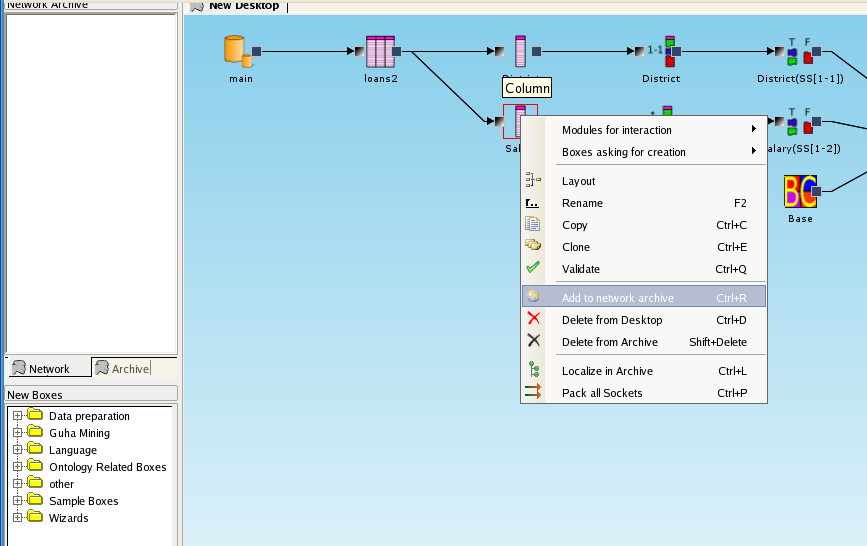
\includegraphics[width=12cm]{add_to_network_archive}
	\caption{Add a connection to the network archive}
\end{figure}
It will ask a user for entering a label after dragging a box from desktop to network archive.
\begin{figure}
	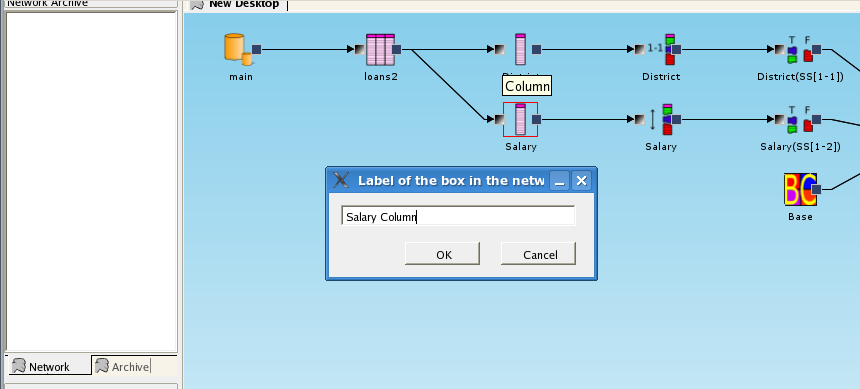
\includegraphics[width=12cm]{set_name_of_box_in_network_archive}
	\caption{Set a name of box in the network archive}
\end{figure}
After that in the list new item with selected label should be visible.
\begin{figure}
	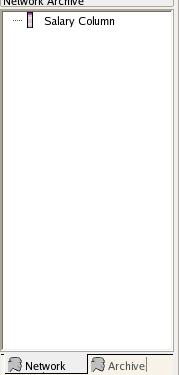
\includegraphics[height=7cm]{network_archive_box_added}
	\caption{New box added to the network archive}
\end{figure}
User can than go to another computer which use the same network archive and drag the box from network archive to another project. It should create a new copy of the box with all it's subboxes on the desktop.
\begin{figure}
	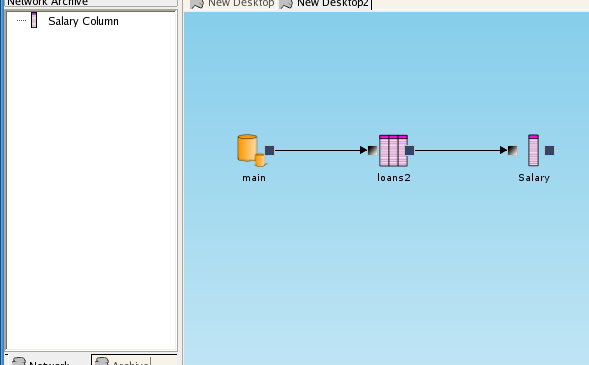
\includegraphics[width=12cm]{network_archive_drop_to_desktop}
	\caption{Drop box to a desktop from the network archive}
\end{figure}
He can also remove the box from the network archive.
\begin{figure}
	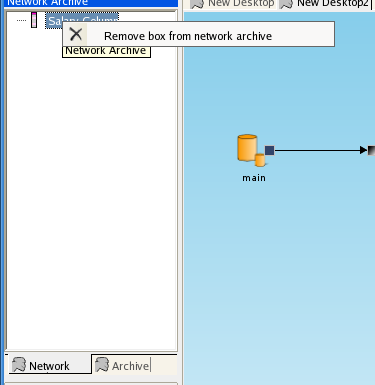
\includegraphics[height=7cm]{network_archive_remove_box}
	\caption{Remove box from the network archive}
\end{figure}

\subsubsection{Future enhancements}
It woul be nice to organize boxes in network archives in some structure. It can be one level structure (labels) or tree structures like directories. Another enhancement would be to add user rights to these labels. Easy thing to do is to allow Ferda FrontEnd to work with more network archives.

\subsubsection{Summary}
Network archive is new place where a user can store connections. It is independent on projects. One network archive can be accessed from more computers. It is way how to move connections from one project to another.


\subsection{Summary}

\section{Language boxes and expresions}
Every programming language has from beggining at least small set of functions. Also it has some way how to use these functions to create more complex ones. Such aparat has been created for ferda as main part of this diploma thesis.

\subsection{Constants}

\subsection{Boxes for math}
Mathematical expressions are really important for programmers, statistics and analitics. Support for them is important. 

\subsubsection{Binary operation}
First 
\begin{figure}
	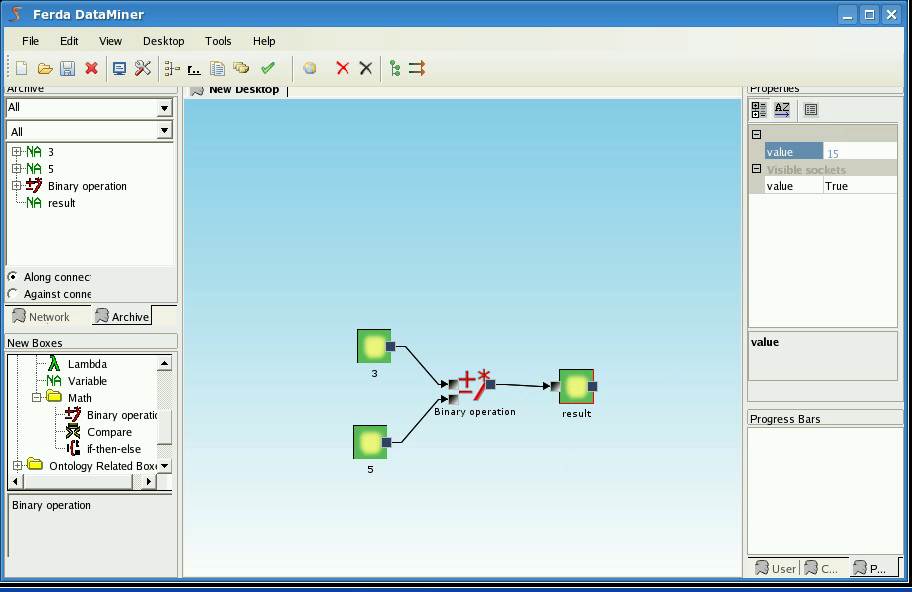
\includegraphics[width=12cm]{binaryOperation2.png}
	\caption{}
\end{figure}

\subsubsection{Comparision}
\begin{figure}
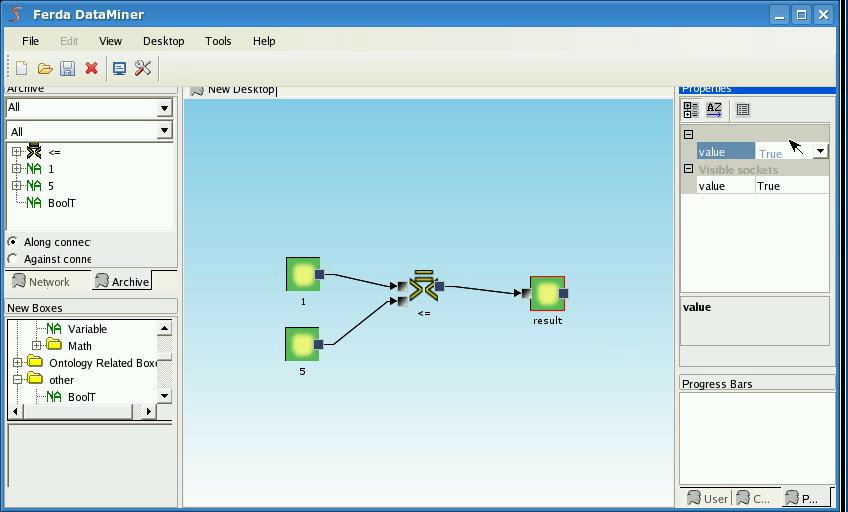
\includegraphics[width=12cm]{compare2.png}
	\caption{}
\end{figure}

\subsubsection{If expressions}
\begin{figure}
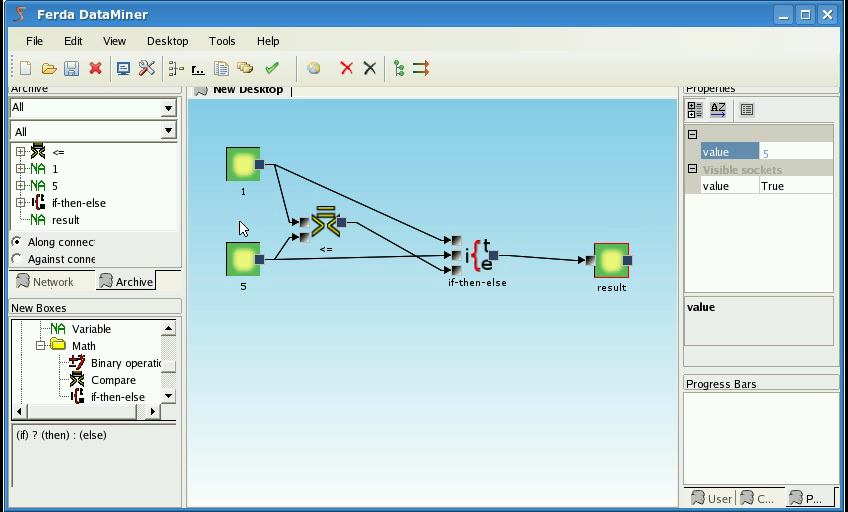
\includegraphics[width=12cm]{ifthenelse2.png}
	\caption{}
\end{figure}

\subsection{Lambda expression}
Basic facts
\begin{itemize}
	\item From lambda calculus $(\lambda x.(1+x))(9)$
	\item Basics of functional programming
\end{itemize}

Lambda in C\# 3
\begin{verbatim}
public delegate int function(int x);

public static void Main(string[] args)
{
  function plusOne = x => 1 + x;
  var a = plusOne(9);
  System.Console.WriteLine(a);
}
\end{verbatim}
	
Other languages

Lambda in F\#
\begin{verbatim}
let onePlus x = 1 + x
do printf "%s" (onePlus(9)) 
\end{verbatim}

Lambda in Python
\begin{verbatim}
plusOne = lambda x: 1 + x
print plusOne(9)
\end{verbatim}

without parameters
\begin{figure}
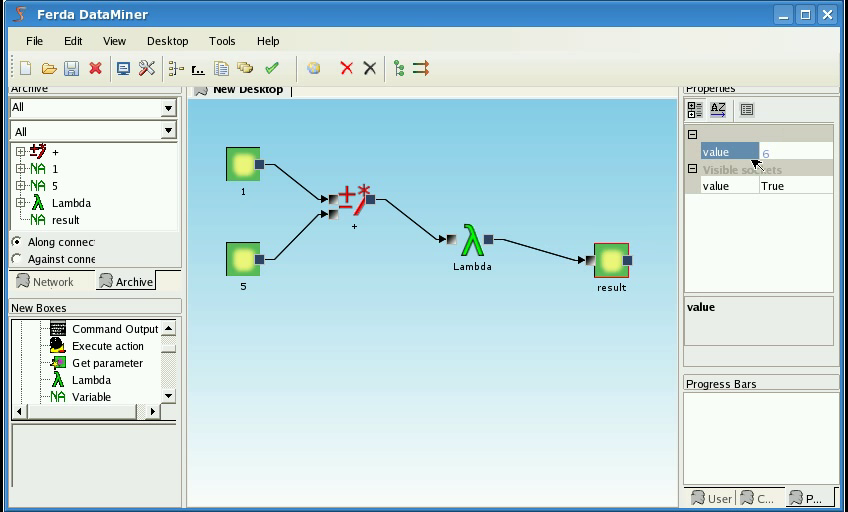
\includegraphics[width=12cm]{lambdaBasic2.png}
	\caption{}
\end{figure}

One constant parameter specified
\begin{figure}
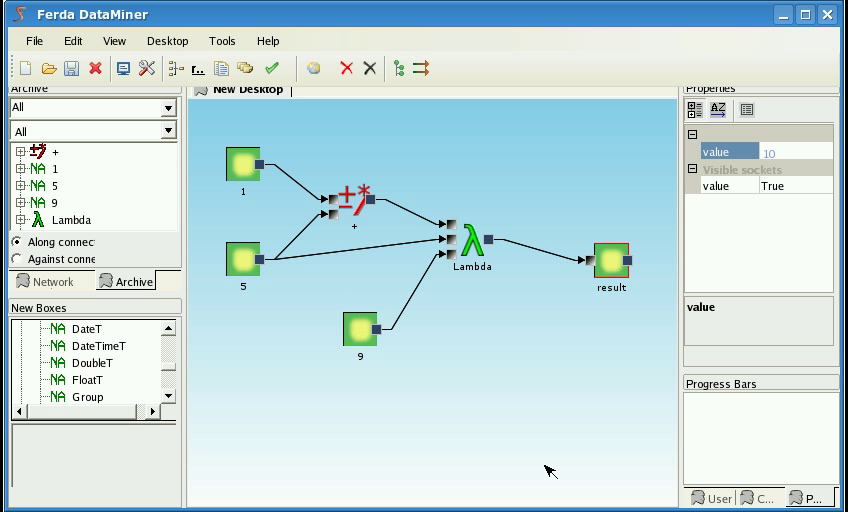
\includegraphics[width=12cm]{lambdaBasic3.png}
	\caption{}
\end{figure}
	
\subsubsection{Implementation of lambda}
How it really works -- Algoritm
\begin{itemize}
	\item Values of variables are cloned (whole subtree)
	\item Main function is cloned with substitution and returned
\end{itemize}

\subsubsection{Example usage of lambda -- factorial}
Factorial in C\# -- Structural version

\begin{verbatim}
public static int Factorial(int x)
{
  if (x == 0)
  {
    return 1;
  }
  else
  {
    return x * Factorial(x - 1);
  }
}
\end{verbatim}
	
Factorial in C\# -- Expresion version

\begin{verbatim}
public static int Factorial2(int x)
{
  return (x == 0) ? 1 : x * Factorial2(x - 1);
}
\end{verbatim}

Factorial in other languages

Python
\begin{verbatim}
fac = lambda x: x == 0 and 1 or x * fac(x - 1)
\end{verbatim}

F\#
\begin{verbatim}
let rec factorial n =
    if n=0 then 1 else n * factorial(n - 1)
\end{verbatim}
	
Factorial in Ferda
\begin{figure}
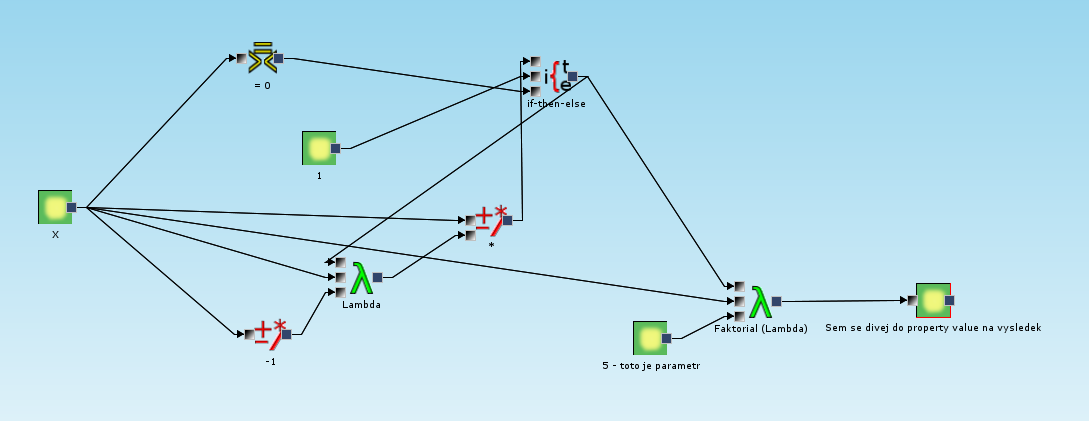
\includegraphics[width=12cm]{faktorial}
	\caption{}
\end{figure}

\subsection{Other new boxes}
\subsubsection{Get parameter}
\begin{figure}
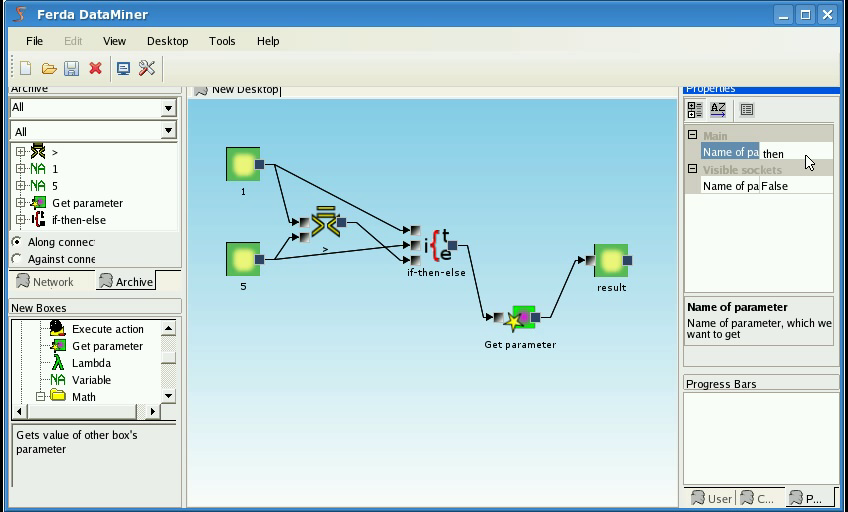
\includegraphics[width=12cm]{getParameter2.png}
	\caption{}
\end{figure}

\subsubsection{Execute action}
\begin{figure}
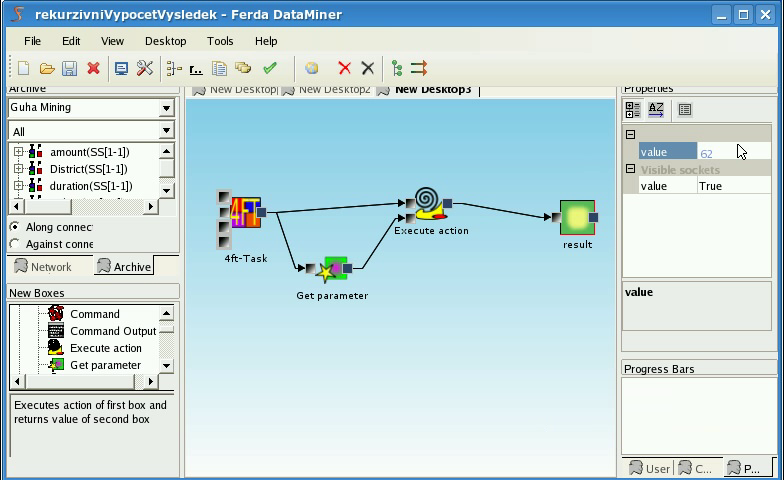
\includegraphics[width=12cm]{executeAction2.png}
	\caption{}
\end{figure}

\subsubsection{Command and command output}
\begin{figure}
	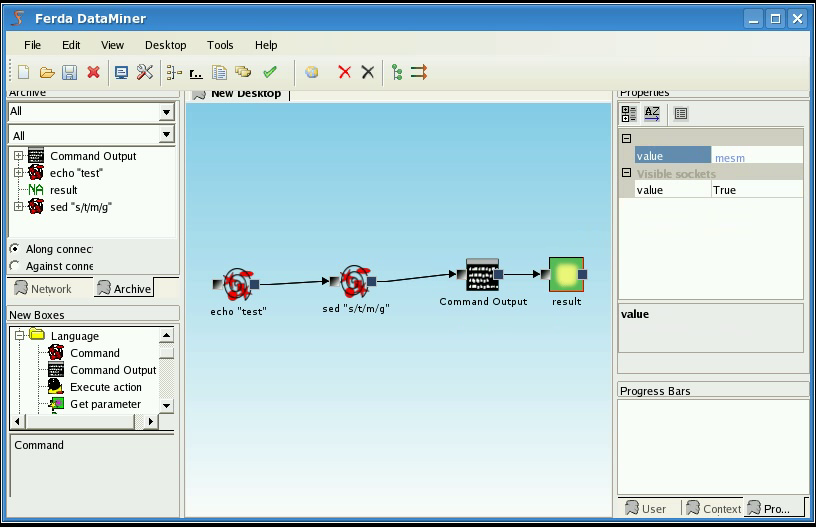
\includegraphics[width=12cm]{command2.png}
	\caption{}
\end{figure}

The same in console
\begin{figure}
	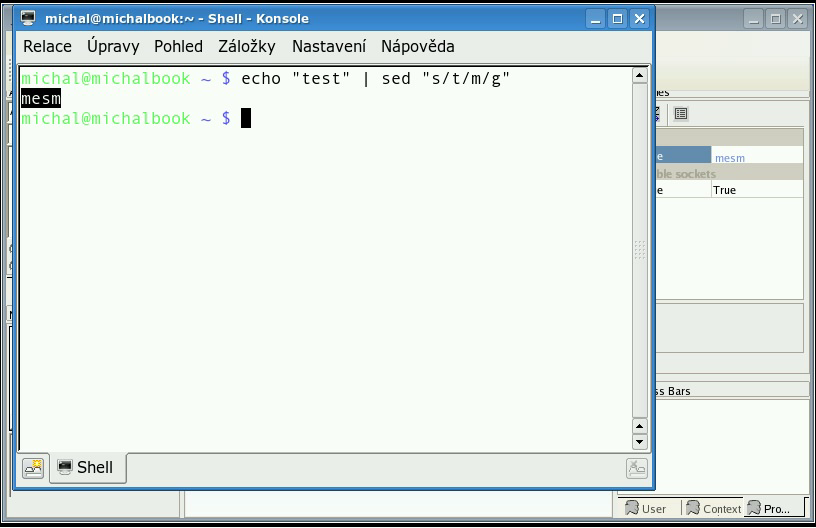
\includegraphics[width=12cm]{command3.png}
	\caption{}
\end{figure}

result browser - aby umel heterogenni vysledky - vystup z 4FT + vystup z CF

Implementation of GUHA in Ferda by 'small' boxes.
\section{Lambda expression}
\section{Sequences}
\section{Examples}
\subsection{Four fold task in recursion}
\subsection{Getting basic information from table}
\section{Implementation details}
\section{Problems in the source code of Ferda}
\section{Advanced tools and topics}
\subsection{Unit tests}
It would be nice to have a box called unit test, which should have a name and one socket for connecting assert boxes. Assert box should be a box which validates some condition and when the condition is not satisfied it should return some message describing the problem. Then there should be small aplication which takes a project as parameter and calls all unit tests in the project. Unit tests should call all asserts which are connected to the test. When any of them fail the application should return the message with name of unit test and the error message from the failed assert. Even though one unit test failed it should call other tests.

Similar is the NUnit tool for .NET Framework. For reusing tools which executes nunit tests it would be nice to create generator of nunit tests from ferda project unit tests. Such enerator should create one assembly for one project, but also so many test methods so many unit test boxes are in the project. There should be one startup method for initializing the Ferda Project Manager and for loading the project. 

\section{Dependency injection}
Dependency injection is modern pattern in object oriented programming. You create a services and specify which services depends on which interfaces and later you set if needed which instances should be used. It is very usefull for unit testing. In Ferda we can see a box with all it's subboxes as a service. Notset sockets are interfaces on which it depends (because of lambda box it is not needed to define it on subboxes).

\section{Aspect oriented programming}
\section{Future tasks to do in ferda}
%popis jednotlivych tasku s narocnosti, uzitkem - bodove ohodnotit

% modules for interacion je treba vylepsit

%vyjimky a Ferda - uzivatel muze chytat a vysilat vyjimky
%vyber na kterem pocitaci ktera krabicka bezi
\end{document}
